\chapter{Założenia projektowe}

Tematem pracy jest stworzenie aplikacji wspomagającej szacowanie historyjek metodą planning pokea.
Aplikacja pozwoli na przeprowadzenie gry, której backlog będzie pochodził z githuba,
 a wyniki będą do niego nadsyłane do githuba.
 Aplikacja będzie synchronizowana z githubem,
czyli że jeżeli jakieś issue będzie z niego usunięte, usięnięte zostanie z gry.
Gra będzie posiadała także możliwości zamknięcia danego issue, edycji itd.
Inną planowaną funkcjonalnością jest możliwość tworzenia własnej skali estymacji.

Nie wszystkie funkcjonalności wymienione powyżej będą zaimplementowane w prototypie aplikacji.
Gracze, będą dodawani do gry przez dzielenie się linkiem,
 oczywiście właściciel będzie mógł gracza wyrzucić z gry.

 Synchronizacja z githuba wymaga wykorzystania webhooków w githubie.
 Jednak aby je zaimplementować w Firebase trzeba zapłacić.

 \section{Wymagania funkcjonalne}

 \begin{itemize}
    \item Logowanie przez githuba
    \item Pobieranie historyjek z Github'a
    \item Synchronizacja z Github'em
    \item Możliwość tworzenia list z issues Github'a
    \item Możliwość tworzenia gry.
    \item Możliwość zapraszania graczy.
    \item Możliwość głosowania przez graczy.
    \item Możliwość tworzenia własnej skali estymacji.
    \item Możliwość komentowania każdej historyjki podczas gry,
    co będzie zsynchronizowane z Github'em.
    \item Możliwość automatycznego przeliczania wyników.
    \item Możliwość wyrzucenia gracza z gry przez właściciela.
    \item Możliwość eksportu wyników gry w postaci historyjek do Github'a.
    \item Każdy gracz powinien być dodawany jako gość, jeśli nie ma konta.
\end{itemize}

\section{Wymagania niefunkcjonalne}

\begin{itemize}
    \item Oprogramowanie musi być responsywne i proste.
    \item Aplikacja powinna się uruchamiać na przeglądarce internetowej.
    \item Aplikacja powinna działać w najnowszych wersjach przeglądarek.
    \item Aplikacja powinna działąć w czasie rzeczywistym.
    \item Serwer powinien obsłużyć  co najmniej 200 połączeń użytkowników.
    \item Zapewnienie bezpieczeństwa danych.
\end{itemize}

\section{Sposób komunikacji}

Aby aplikacja mogła komunikować się w czasie rzeczywistym niezbędne jest wykorzystanie websocketów. Rys
~\ref{rys:websocket}.

\begin{figure}[H]
	\centering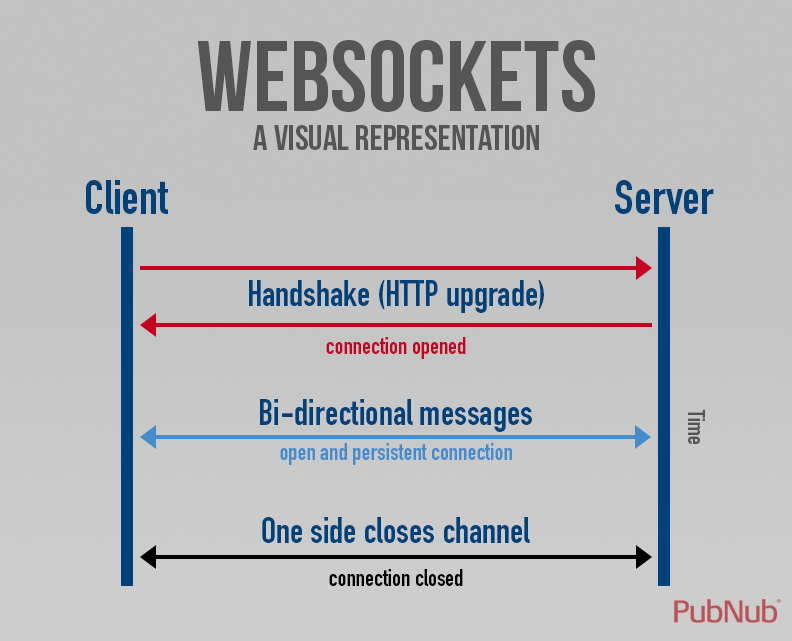
\includegraphics[width=.6\textwidth]{img/websocket}
	\caption{websockets}.
	\label{rys:websocket}
\end{figure}

\section{Wykorzystanie technologie}

Aplikacja zostanie napisana w języku JavaScript z wykorzystaniem scss, jsx i html.
Wybór technologii jest moim zdaniem doskonały pod ReactJS

Wybrany stack technologiczny to:
\begin{itemize}
    \item Node.Js - środowisko uruchomieniowe do tworzenia aplikacji.
    \item Yarn - Manadżer pakietów.
    \item React -  biblioteka front-end do tworzenia interfejsów.
    \item Redux - architektura wspomagająca zarządzanie stanem aplikacji.
    \item Bootstrap - framework pomagający tworzyć wygląd strony.
    \item Webpack - narzędzie do opakowywania, kompilowania i minimalizowania kodu.
    \item Firebase - platforma służąca jako backend aplikacji.
\end{itemize}